\documentclass[11pt]{article}
% Explicación de la frecuencia instantánea y el chirp (apoyo al problema 7 del taller de repaso, Examen 1).
% Figuras: python figuras_chirp.py  (Python de Windows, el que tiene numpy/matplotlib).
% Compilar con XeLaTeX (dos pasadas):  xelatex explicacion-frecuencia-instantanea.tex
\usepackage[spanish,es-noshorthands,es-nodecimaldot,es-tabla]{babel}
\usepackage{fontspec}
\usepackage{amsmath,amssymb,mathtools}
\usepackage{booktabs,array}
\usepackage{graphicx}
\usepackage{xcolor}
\usepackage{enumitem}
\usepackage[letterpaper,margin=2.2cm,top=2.2cm,bottom=2.2cm]{geometry}
\usepackage{titlesec}
\usepackage{fancyhdr}
\usepackage[most]{tcolorbox}
\usepackage{float}
\usepackage[font=small,labelfont=bf,labelsep=period]{caption}
\usepackage{hyperref}
\hypersetup{colorlinks=true,linkcolor=black,urlcolor=black}

\definecolor{tema}{RGB}{20,60,120}
\definecolor{caja}{RGB}{235,241,250}
\definecolor{nota}{RGB}{245,245,235}
\definecolor{alerta}{RGB}{170,30,30}
\titleformat{\section}{\Large\bfseries\color{tema}}{\thesection.}{0.5em}{}[\vspace{-0.4ex}\color{tema}\rule{\linewidth}{0.8pt}]
\titleformat{\subsection}{\large\bfseries\color{tema}}{\thesubsection}{0.5em}{}
\titlespacing*{\section}{0pt}{3ex}{1.5ex}
\titlespacing*{\subsection}{0pt}{2.2ex}{0.8ex}
\setlist{itemsep=0.3ex,topsep=0.6ex,leftmargin=1.5em}
\setlength{\parindent}{0pt}
\setlength{\parskip}{0.9ex}
\pagestyle{fancy}\fancyhf{}
\lhead{\small Óptica No Lineal 2026-II — Frecuencia instantánea y chirp}
\rhead{\small p.~\thepage}
\renewcommand{\headrulewidth}{0.4pt}
\setlength{\headheight}{14pt}

\newcommand{\jj}{\mathrm{j}}
\newcommand{\ojo}[1]{{\color{alerta}\textbf{Ojo:} #1}}
\newtcolorbox{clave}[1][]{enhanced,breakable,colback=caja,colframe=tema,boxrule=0.5pt,arc=2pt,
  left=6pt,right=6pt,top=4pt,bottom=4pt,fonttitle=\bfseries\small,#1}
\newtcolorbox{idea}[1][]{enhanced,breakable,colback=nota,colframe=black!25,boxrule=0.4pt,arc=2pt,
  left=6pt,right=6pt,top=3pt,bottom=3pt,fonttitle=\bfseries\small,coltitle=black,colbacktitle=black!8,#1}

\begin{document}

\begin{center}
{\LARGE\bfseries\color{tema} Frecuencia instantánea y chirp}\\[1ex]
{\large Cómo leer un pulso en el tiempo y en la frecuencia}\\[1ex]
{\small Apoyo al problema 7 del taller de repaso del Examen 1 (Saleh \& Teich, \emph{Fundamentals of Photonics}, 2.ª ed., §22.1 y §22.3; §5.6)\\
Juan E. Rodríguez Ochoa · UNAL · 2026-11-15}
\end{center}

\begin{idea}[title={Las dudas que motivan este documento}]
\begin{enumerate}[leftmargin=1.6em]
\item Si un pulso tiene muchas frecuencias a la vez, ¿qué significa que $\nu_i(t)$ sea \emph{la} frecuencia en el instante $t$?
\item ¿Qué quiere decir que una frecuencia «domina» en un instante?
\item Cada componente de frecuencia es una onda monocromática que se extiende de $-\infty$ a $+\infty$ (sin localidad). Entonces, ¿cómo puede una frecuencia «llegar primero»?
\item ¿Es válido pensar el tiempo como una posición en el espacio? ¿Cuál es la referencia?
\item ¿Es el chirp solo la acumulación de dispersión, es decir, ensanchamiento?
\end{enumerate}
\end{idea}

%=====================================================================
\section*{Convenciones y parámetros}
%=====================================================================
Se usa la convención de Saleh ($e^{+\jj\omega t}$) y el campo del problema 7:
\[
f(t)=e^{-t^2/\tau^2}\,e^{\jj\phi(t)},\qquad \phi(t)=2\pi\nu_0t+bt^2,\qquad
\mathcal E(z,t)=\mathrm{Re}\{f(t-z/c_0)\}\,\hat{\mathbf x}.
\]
Parámetros del enunciado: $\tau=20$ fs, $\nu_0=375$ THz ($\lambda_0=799$ nm, periodo óptico $T_0=2.67$ fs), $b=5\times10^{27}$ s$^{-2}$. El parámetro de chirp de Saleh (22.1-5) es
\[
a=b\tau^2=2 .
\]
Transformada de Fourier (para pasar entre el tiempo y la frecuencia):
\[
\tilde A(\nu)=\int_{-\infty}^{\infty}f(t)\,e^{-\jj2\pi\nu t}\,dt,\qquad f(t)=\int_{-\infty}^{\infty}\tilde A(\nu)\,e^{+\jj2\pi\nu t}\,d\nu .
\]
$|\tilde A(\nu)|^2$ es el \textbf{espectro}; el argumento $\psi(\nu)=\arg\tilde A(\nu)$ es la \textbf{fase espectral}. Todas las figuras se generaron con \texttt{figuras\_chirp.py} (misma carpeta); los colores se mantienen en todo el documento: \textcolor[RGB]{214,69,69}{rojo} = frecuencia baja o instante temprano, \textcolor[RGB]{27,175,122}{verde} = centro, \textcolor[RGB]{42,120,214}{azul} = frecuencia alta o instante tardío.

%=====================================================================
\section{Respuesta corta}
%=====================================================================
\begin{clave}[title={Tres ideas}]
\begin{enumerate}[leftmargin=1.6em]
\item \textbf{Un pulso no es una onda monocromática: es una suma de ondas monocromáticas eternas}, cuya interferencia se cancela casi por completo fuera del pulso y se refuerza dentro de él. La localización en el tiempo no viene de ninguna componente, sino de \emph{cómo se suman}, es decir, de sus \textbf{fases relativas}.
\item \textbf{$\nu_i(t)$ no es «una de esas ondas que llega».} Es la rapidez con que oscila el \emph{campo total} (la suma) alrededor del instante $t$: $\nu_i=\frac{1}{2\pi}\,d\phi/dt$. Es una propiedad de la señal ya sumada, no de una componente.
\item \textbf{El espectro y $\nu_i(t)$ describen el mismo campo.} El espectro dice \emph{qué frecuencias hay en total}; $\nu_i(t)$ dice \emph{en qué orden aparecen en el tiempo}. El chirp es justamente que ese orden existe: la frecuencia local cambia a lo largo del pulso, $\nu_i(t)\neq\text{cte}$.
\end{enumerate}
\end{clave}

Lo que sigue desarrolla cada idea con ecuaciones y figuras.

%=====================================================================
\section{Las ondas monocromáticas no tienen localidad, y aun así hay pulsos}
%=====================================================================
\subsection{Un pulso como suma de ondas eternas}
La fórmula de síntesis de Fourier,
\[
f(t)=\int\tilde A(\nu)\,e^{\jj2\pi\nu t}\,d\nu,
\]
dice que el pulso es una superposición de ondas $e^{\jj2\pi\nu t}$, cada una con amplitud constante para \emph{todo} $t$ (Fig.~\ref{fig:comp}). La objeción es correcta: ninguna de esas ondas «llega» ni «se va»; todas están presentes siempre. Entonces, ¿de dónde sale un pulso que existe solo durante unas decenas de femtosegundos?

De la \textbf{interferencia}. La Fig.~\ref{fig:suma} suma las componentes de la Fig.~\ref{fig:comp} progresivamente:

\begin{itemize}
\item \textbf{(a)} Con una sola componente hay una onda de amplitud constante y no hay pulso.
\item \textbf{(b), (c)} Al añadir componentes cercanas aparece una zona central de amplitud mayor: ahí las componentes están en fase y se suman; lejos del centro quedan desfasadas y se cancelan parcialmente.
\item \textbf{(d)} Con todo el espectro (81 componentes) el pulso queda perfectamente localizado: fuera de $|t|\gtrsim40$ fs la suma es cero.
\item \textbf{(e)} Con los \emph{mismos módulos} pero \textbf{fases al azar} no hay pulso: se obtiene un ruido que llena toda la ventana.
\end{itemize}

\begin{figure}[H]\centering
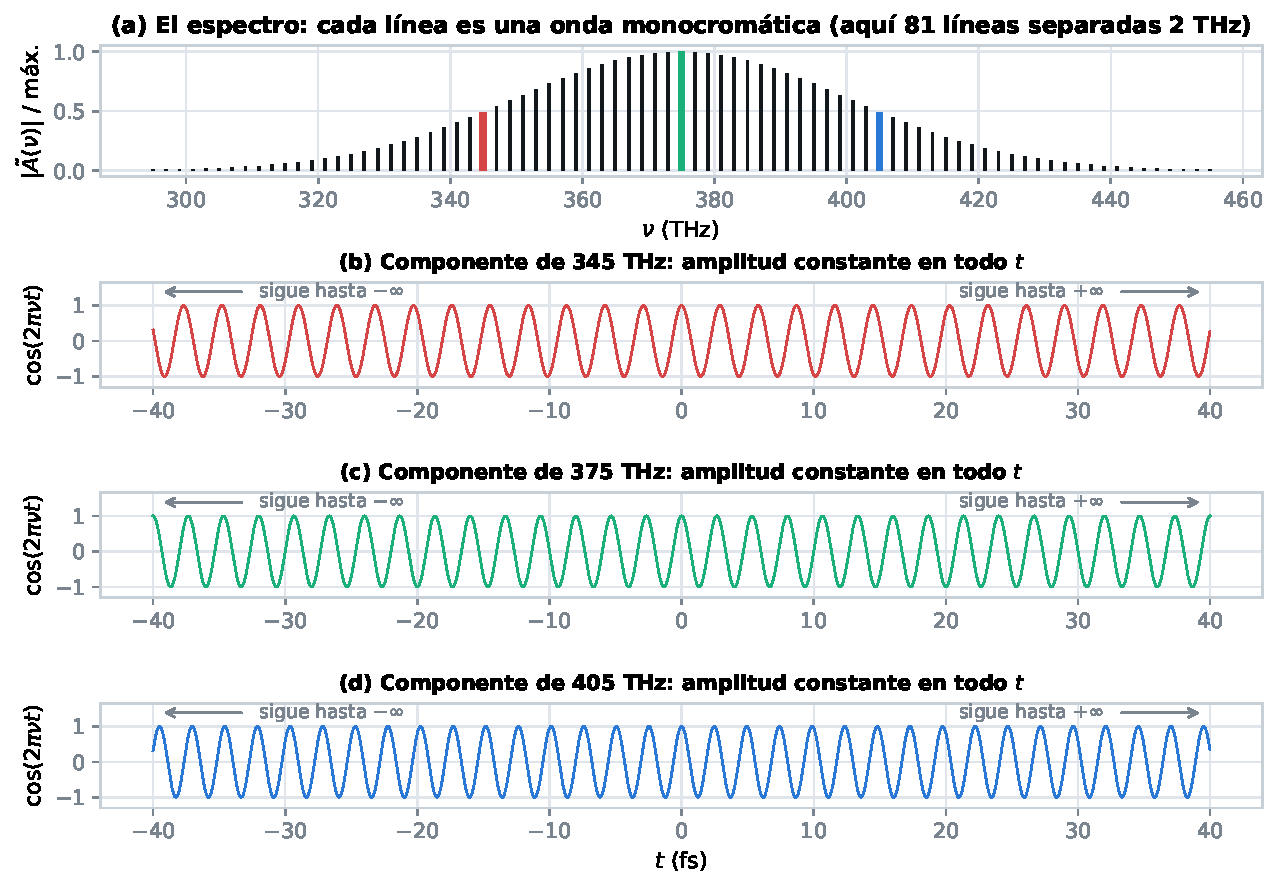
\includegraphics[width=\linewidth]{figuras/fig02_componentes_eternas.pdf}
\caption{Espectro del pulso del problema 7 muestreado en 81 líneas (separadas 2 THz) y tres de sus componentes. Cada componente es una onda monocromática de amplitud constante en todo instante.}\label{fig:comp}
\end{figure}

\begin{figure}[H]\centering
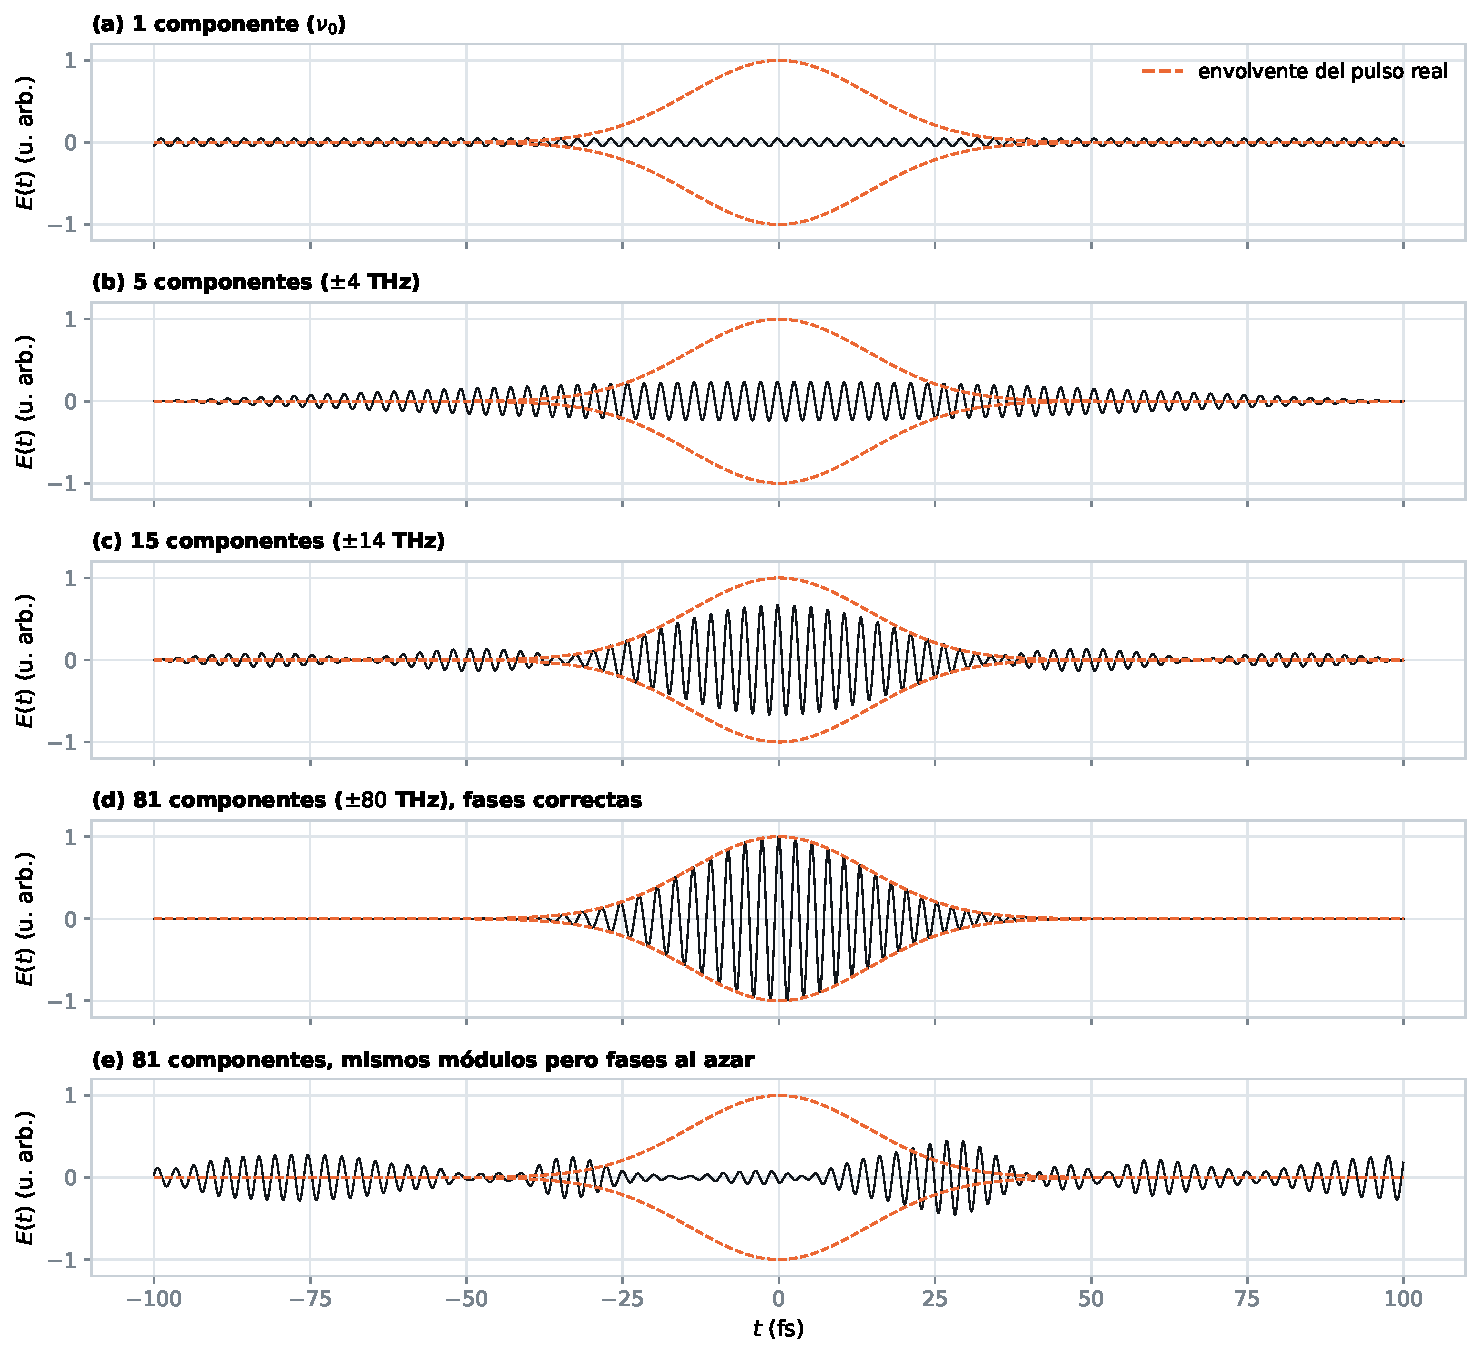
\includegraphics[width=\linewidth]{figuras/fig03_suma_y_localizacion.pdf}
\caption{Suma progresiva de componentes. La línea discontinua naranja es la envolvente del pulso real. Con las 81 componentes y sus fases correctas (d) se reproduce el pulso (error máximo $1.2\times10^{-3}$ frente a $f(0)=1$); con los mismos módulos y fases al azar (e) no hay pulso.}\label{fig:suma}
\end{figure}

\begin{clave}[title={Qué se concluye}]
\begin{itemize}[leftmargin=1.2em]
\item El \emph{cuándo} está codificado en la \textbf{fase espectral} $\psi(\nu)$, no en el módulo $|\tilde A(\nu)|$: dos pulsos con el mismo espectro pueden ser totalmente distintos en el tiempo (ver §\ref{sec:disp}).
\item Para localizar la energía en un intervalo $\Delta t$ hace falta un ancho de banda $\Delta\nu\gtrsim1/\Delta t$. Para un gaussiano sin chirp, $\Delta\nu_{\rm FWHM}\,\tau_{\rm FWHM}=0.44$.
\end{itemize}
\end{clave}

\subsection{Cómo es el espectro del pulso con chirp}
Se escribe $f(t)=e^{\jj2\pi\nu_0t}e^{-\alpha t^2}$ con $\alpha=(1-\jj a)/\tau^2$ (porque $-t^2/\tau^2+\jj bt^2=-(1-\jj b\tau^2)\,t^2/\tau^2$). La integral gaussiana $\int e^{-\alpha t^2-\jj\omega t}dt=\sqrt{\pi/\alpha}\,e^{-\omega^2/4\alpha}$, con $\omega=2\pi(\nu-\nu_0)$, da
\[
\tilde A(\nu)=\sqrt{\frac{\pi}{\alpha}}\;\exp\!\Big[-\frac{\pi^2(\nu-\nu_0)^2}{\alpha}\Big],\qquad \frac1\alpha=\frac{\tau^2(1+\jj a)}{1+a^2}.
\]
Separando módulo y fase:
\begin{equation}\label{eq:espectro}
|\tilde A(\nu)|^2\propto\exp\!\Big[-\frac{2\pi^2\tau^2(\nu-\nu_0)^2}{1+a^2}\Big],\qquad
\psi(\nu)=-\frac{\pi^2\tau^2\,a\,(\nu-\nu_0)^2}{1+a^2}+\text{cte}.
\end{equation}
Dos consecuencias:
\begin{itemize}
\item \textbf{Un chirp lineal en el tiempo es una fase espectral cuadrática}: $\psi\propto(\nu-\nu_0)^2$. Es la misma estructura que en la dispersión (§\ref{sec:disp}).
\item \textbf{El chirp ensancha el espectro sin cambiar la duración}: el FWHM espectral es $\sqrt{1+a^2}$ veces el del pulso sin chirp. Con $\tau=20$ fs: $18.7$ THz si $a=0$ y $18.7\sqrt5=41.9$ THz si $a=2$.
\end{itemize}

%=====================================================================
\section{Qué es exactamente la frecuencia instantánea}
%=====================================================================
Se mira el campo real cerca de un instante $t$: $\mathrm{Re}\{f\}=e^{-t^2/\tau^2}\cos\phi(t)$. Si la envolvente cambia despacio (aquí $\tau=20$ fs frente a $T_0=2.67$ fs: unos 7 ciclos por $\tau$), la parte que oscila es $\cos\phi(t)$, y la rapidez con que su argumento avanza es la \textbf{frecuencia local}:
\[
\nu_i(t)=\frac1{2\pi}\frac{d\phi}{dt}=\frac1{2\pi}\big(2\pi\nu_0+2bt\big)=\nu_0+\frac{b\,t}{\pi}.
\]
Es la misma idea que la velocidad: la derivada de la posición da la velocidad, y la derivada de la fase da la frecuencia. Equivale a decir que \textbf{entre dos crestas consecutivas pasa un tiempo} $T_i(t)\simeq1/\nu_i(t)$.

La Fig.~\ref{fig:inst} lo muestra. En (c1)--(c3) cada ventana tiene 12 fs y se ve el mismo número de ciclos, pero con periodos distintos: $2.98$ fs en $t=-25$ fs (335 THz), $2.67$ fs en el centro (375 THz) y $2.41$ fs en $t=+25$ fs (415 THz). Entre $t=-\tau$ y $t=+\tau$ la frecuencia pasa de $343.2$ a $406.8$ THz, un barrido de $2b\tau/\pi=63.7$ THz.

\begin{figure}[H]\centering
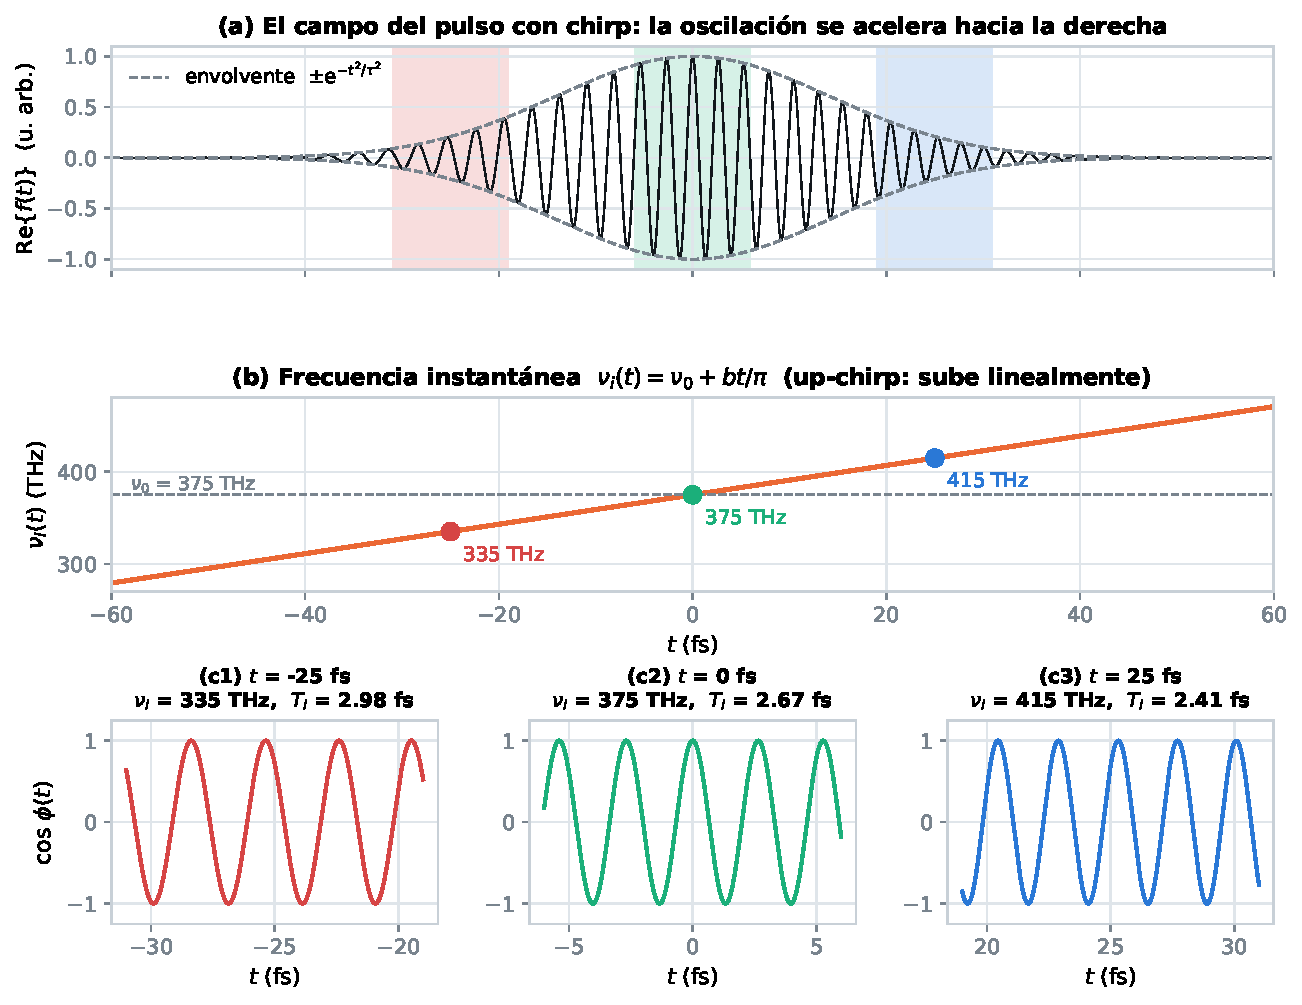
\includegraphics[width=\linewidth]{figuras/fig01_campo_y_frecuencia_instantanea.pdf}
\caption{(a) Campo del pulso del problema 7. (b) Frecuencia instantánea $\nu_i(t)=\nu_0+bt/\pi$. (c) Ampliaciones de las tres ventanas sombreadas en (a): se grafica $\cos\phi(t)$ para ver solo la oscilación; el periodo local es $T_i=1/\nu_i$.}\label{fig:inst}
\end{figure}

\ojo{$\nu_0$ y $\nu_i(t)$ son cosas distintas. $\nu_0$ es el \emph{centro del espectro}; $\nu_i(t)$ es la frecuencia \emph{local}. Coinciden en un solo instante, $t=0$. Si se promedia $\nu_i(t)$ con el peso de la intensidad se recupera $\nu_0$.}

%=====================================================================
\section{¿Qué significa que una frecuencia «domina» en el instante $t$?}
%=====================================================================
«Domina» no quiere decir que sea la única presente ni que sea una onda eterna que aparece en $t$. Tiene un significado operativo: si se observa el campo \textbf{a través de una ventana corta} centrada en $t$ y se calcula su espectro, ese \textbf{espectro local} tiene un pico, y el pico está en $\nu_i(t)$.

Formalmente, con una ventana gaussiana $w(t'-t)=e^{-(t'-t)^2/2\sigma_w^2}$:
\[
S(t,\nu)=\Big|\int f(t')\,w(t'-t)\,e^{-\jj2\pi\nu t'}\,dt'\Big|^2 .
\]
A esa función de $(t,\nu)$ se le llama \emph{espectrograma}. La Fig.~\ref{fig:espectro} la muestra para dos anchos de ventana.

\begin{figure}[H]\centering
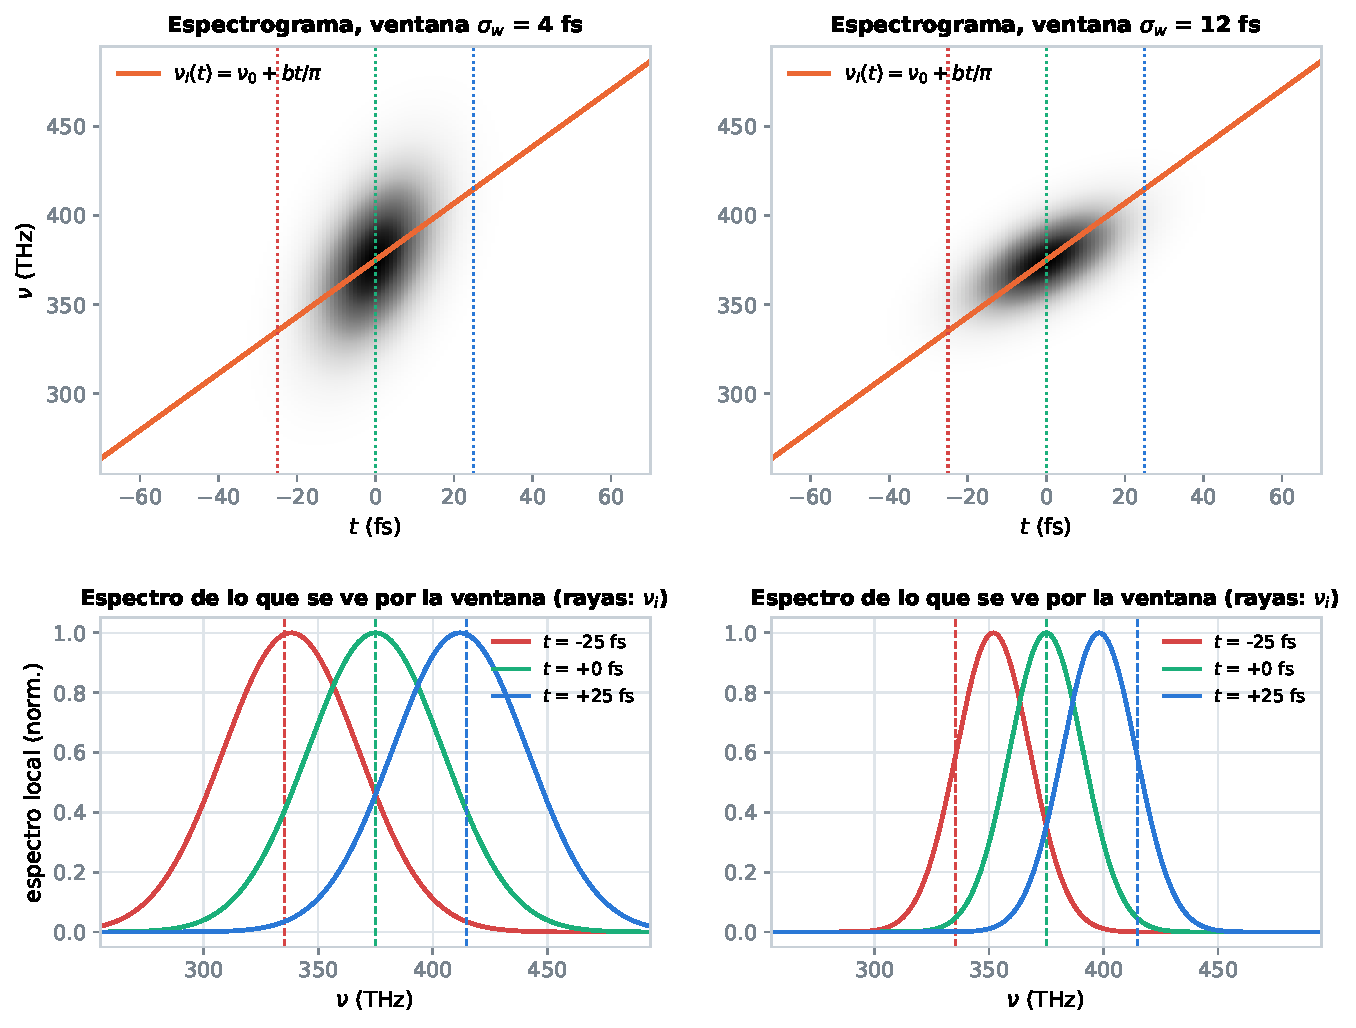
\includegraphics[width=0.95\linewidth]{figuras/fig04_espectro_local.pdf}
\caption{Espectrograma del pulso del problema 7 con ventana corta ($\sigma_w=4$ fs, izquierda) y larga ($\sigma_w=12$ fs, derecha). Arriba: mapa $S(t,\nu)$ y la recta $\nu_i(t)$. Abajo: cortes en $t=-25,\,0,\,+25$ fs; las rayas son $\nu_i(t)$.}\label{fig:espectro}
\end{figure}

Hay que leer la figura con cuidado, porque muestra el compromiso entre ver «un instante» y ver una frecuencia definida:
\begin{itemize}
\item \textbf{Ventana corta} ($\sigma_w=4$ fs): el pico está casi sobre $\nu_i(t)$ (412 THz en $t=25$ fs, frente a 415 THz), pero es \textbf{muy ancho} (unos 70 THz): en 4 fs no caben suficientes ciclos para definir una frecuencia con precisión.
\item \textbf{Ventana larga} ($\sigma_w=12$ fs): el pico es \textbf{más angosto} (unos 38 THz), pero se \textbf{sesga hacia el centro del pulso} (398 THz en $t=25$ fs): la ventana promedia lo que ocurre en un intervalo largo y la frecuencia deja de ser «de ese instante».
\end{itemize}
El sesgo tiene fórmula. El producto de la ventana por el pulso es un gaussiano cuyo centro temporal es $t_c=\kappa\,t$, con
\[
\kappa=\frac{1/(2\sigma_w^2)}{1/\tau^2+1/(2\sigma_w^2)},
\]
y el pico del espectro local está en $\nu_0+\kappa\,bt/\pi$. Con $\tau=20$ fs: $\kappa=0.93$ para $\sigma_w=4$ fs y $\kappa=0.58$ para $\sigma_w=12$ fs, lo que reproduce los 412 y 398 THz de la figura.

\begin{clave}[title={Qué es $\nu_i(t)$ en este lenguaje}]
$\nu_i(t)$ es el pico del espectro local \textbf{en el límite de ventana tan corta como se quiera} (donde el pico es fiel al instante), \emph{pero} en ese límite el pico se ensancha sin cota. Es una relación de incertidumbre: no existe una «frecuencia de un instante» con precisión arbitraria, solo una frecuencia local con una resolución $\delta\nu\gtrsim1/\delta t$. Por eso conviene usar $\nu_i(t)$ solo cuando la envolvente varía despacio frente al periodo óptico, como ocurre aquí.
\end{clave}

%=====================================================================
\section{La imagen espacial sí funciona}
%=====================================================================
Pensar el tiempo como posición es válido, y no es solo una metáfora. En el vacío el campo depende de $t$ y $z$ solo por la combinación
\[
u=t-\frac{z}{c_0}:\qquad \mathcal E(z,t)=\mathrm{Re}\{f(u)\}.
\]
El pulso es una \emph{forma} en la variable $u$ que viaja rígida. Esto da dos maneras equivalentes de mirarlo (Fig.~\ref{fig:espacio}):

\begin{itemize}
\item \textbf{Referencia fija en el espacio} (un detector en $z_d$): se registra $\mathcal E(z_d,t)$ y $t$ es el instante de llegada. Lo primero que llega es el \emph{frente}.
\item \textbf{Referencia fija en el tiempo} (una «foto» en $t_0$): se obtiene $\mathcal E(z,t_0)=\mathrm{Re}\{f(t_0-z/c_0)\}$ y $z=c_0(t_0-u)$. El frente está en $z$ grande, y el eje queda \textbf{invertido} respecto al del tiempo.
\end{itemize}
La «referencia invisible» es esta coordenada $u$: el detector fijo en $z_d$, o equivalentemente el propio pulso al que se le asigna el origen $u=0$.

La frecuencia instantánea se traduce en un \textbf{número de onda local}. Con la fase $\Phi(z,t)=2\pi\nu_0u+bu^2$:
\[
\omega_i=\frac{\partial\Phi}{\partial t}=2\pi\nu_0+2bu,\qquad
k_i=-\frac{\partial\Phi}{\partial z}=\frac{2\pi\nu_0+2bu}{c_0}\;\Rightarrow\;\lambda_i(z)=\frac{c_0}{\nu_i(t_0-z/c_0)} .
\]
En la foto con $t_0=0$: en $z=+6\ \mu$m ($u=-20$ fs, frente) $\nu_i=343.1$ THz y $\lambda_i=0.874\ \mu$m (rojo, longitud de onda larga); en $z=-6\ \mu$m ($u=+20$ fs, cola) $\nu_i=406.9$ THz y $\lambda_i=0.737\ \mu$m (azul). Es la misma información que en el tiempo, vista al revés.

\begin{figure}[H]\centering
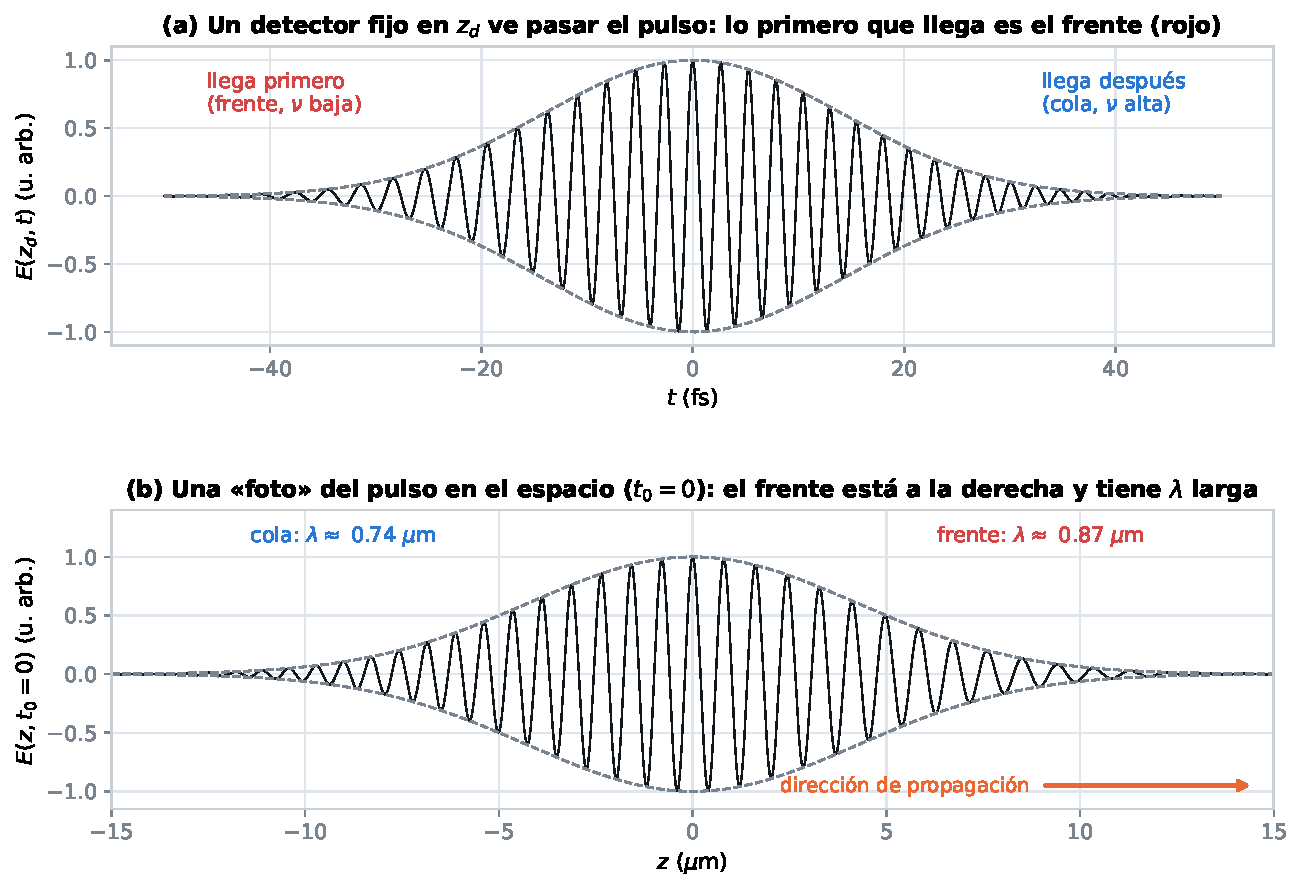
\includegraphics[width=\linewidth]{figuras/fig07_tiempo_y_espacio.pdf}
\caption{El mismo pulso visto (a) en el tiempo, con un detector fijo, y (b) en el espacio, en una «foto» a $t_0=0$. En (b) el eje $z$ tiene el sentido inverso al de $t$: el frente (rojo, $\lambda$ larga) queda a la derecha. Escala: $c_0\tau=6\ \mu$m.}\label{fig:espacio}
\end{figure}

En el vacío esta forma viaja sin deformarse, porque \emph{todas} las componentes de frecuencia van a $c_0$ y mantienen sus fases relativas, por lo que el chirp no cambia. En un medio dispersivo cada frecuencia va a su propia velocidad, las fases relativas cambian y la forma se deforma: ese es el tema de la siguiente sección.

%=====================================================================
\section{Dónde nace el chirp: la dispersión como filtro de fase}\label{sec:disp}
%=====================================================================
Un pulso gaussiano sin chirp, $A(0,t)=e^{-t^2/\tau_0^2}$, se propaga en un medio de dispersión normal ($D_\nu>0$). En el dominio de la frecuencia, el medio multiplica cada componente por una fase que depende de $\nu$ (Saleh §22.3, §5.6):
\[
\tilde A(z,\nu)=\tilde A(0,\nu)\,e^{-\jj\pi D_\nu\nu^2z}=\tilde A(0,\nu)\,\exp\!\big[-\jj\pi^2\tau_0^2\,s\,(\nu-\nu_0)^2\big],\qquad s=\frac{z}{z_0},\quad z_0=\frac{\pi\tau_0^2}{|D_\nu|}.
\]
Es un \textbf{filtro de fase pura}: no cambia $|\tilde A(\nu)|^2$, solo las fases relativas. Es la fase espectral cuadrática de (\ref{eq:espectro}). Con $a(z)=s$ y $\tau(z)=\tau_0\sqrt{1+s^2}$, el pulso queda
\[
A(z,t)\propto\exp\!\Big[-\frac{(1-\jj s)\,t^2}{\tau_0^2(1+s^2)}\Big]\;\Rightarrow\;
\nu_i(t)-\nu_0=\frac{s}{\pi\tau_0^2(1+s^2)}\,t .
\]
La Fig.~\ref{fig:disp} lo comprueba numéricamente, con una FFT del pulso y el filtro de fase, para $s=0,\,1,\,4$ ($\tau_0=20$ fs): el espectro es idéntico en las tres columnas, la duración pasa de 20 a 28 y a 82 fs, y $\nu_i(t)$ coincide con la fórmula analítica.

\begin{figure}[H]\centering
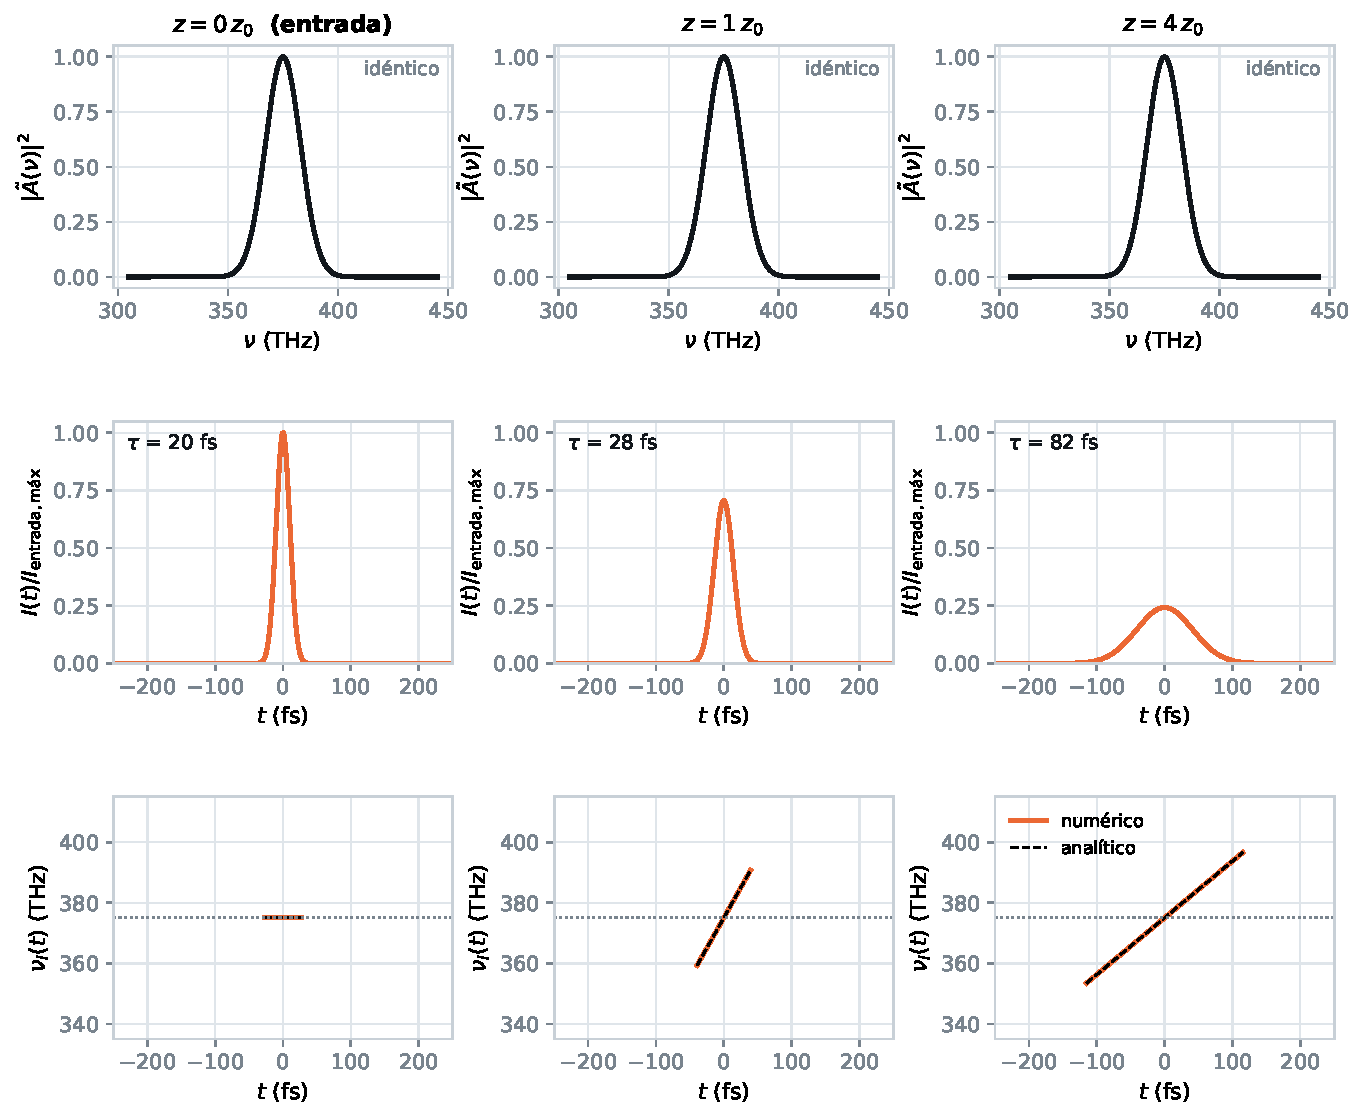
\includegraphics[width=\linewidth]{figuras/fig08_dispersion_solo_fases.pdf}
\caption{Propagación de un pulso sin chirp ($\tau_0=20$ fs, $\nu_0=375$ THz) en dispersión normal, a $z=0,\,z_0,\,4z_0$. Arriba: espectro (idéntico). Centro: intensidad. Abajo: $\nu_i(t)$ numérica y analítica (donde $I$ supera el 2\,\% del máximo).}\label{fig:disp}
\end{figure}

Esto responde a la pregunta sobre qué es el chirp:
\begin{itemize}
\item \textbf{El chirp es la fase del pulso; el ensanchamiento es su consecuencia.} La dispersión introduce el chirp ($a=s$ crece con la distancia) y, con él, el pulso se alarga.
\item \textbf{El chirp puede existir sin dispersión previa.} En el problema 7 está dado desde $z=0$ ($a=2$). Un pulso con chirp puede incluso \emph{comprimirse} en un medio cuya dispersión tenga el signo contrario.
\item \textbf{Las frecuencias se ordenan en el tiempo.} En dispersión normal las frecuencias altas viajan más lento: $\nu_i(t)$ crece con $t$ (up-chirp, $a>0$), con el rojo al frente y el azul atrás, como en el problema 7 y en el 17c.
\item A $z=z_0$ la \emph{pendiente} $d\nu_i/dt$ es máxima ($s/(1+s^2)$ vale $\tfrac12$); después disminuye, pero el \emph{barrido total} sobre el pulso, $\Delta\nu_i\to1/(\pi\tau_0)=15.9$ THz por lado, tiende al ancho del espectro: cuando $s\gg1$ cada frecuencia ocupa su propio tramo del pulso, es decir, el espectro queda «desplegado» en el tiempo.
\end{itemize}

%=====================================================================
\section{¿Qué frecuencia llega primero? La prueba del filtro}
%=====================================================================
Con ondas estrictamente monocromáticas la pregunta no tiene sentido: una onda eterna no tiene hora de llegada. La pregunta se vuelve legítima si se pasa a una \textbf{banda estrecha} de frecuencias: un grupo de componentes vecinas se suma en fase solo en una zona del tiempo, es decir, forma un \textbf{paquete de ondas localizado}, y el paquete sí tiene hora de llegada.

\textbf{Dónde está el paquete.} Cada componente aporta la fase $\psi(\nu)+2\pi\nu t$. Las componentes vecinas se refuerzan cuando esa fase es estacionaria respecto a $\nu$, es decir, cuando
\[
\frac{d\psi}{d\nu}+2\pi t=0\;\Longrightarrow\;t_g(\nu)=-\frac1{2\pi}\frac{d\psi}{d\nu}\qquad(\text{retardo de grupo}).
\]
Para (\ref{eq:espectro}) y para el filtro de fase de la §\ref{sec:disp} sale
\begin{align*}
t_g(\nu)&=\frac{\pi\tau^2a}{1+a^2}\,(\nu-\nu_0)&&\text{(pulso con chirp inicial)},\\
t_g(\nu)&=\pi\tau_0^2\,s\,(\nu-\nu_0)=D_\nu z\,(\nu-\nu_0)&&\text{(tras propagar)}.
\end{align*}
La segunda es el retardo $z/v(\nu)$ de Saleh: cada banda llega con el retraso que le impone la dispersión.

\textbf{El experimento} (Fig.~\ref{fig:filtro}). Se toma el pulso de la Fig.~\ref{fig:disp} en $z=4z_0$ y se hacen pasar por filtros gaussianos estrechos ($\sigma_f=4$ THz) centrados en $\nu_0-15$, $\nu_0$ y $\nu_0+15$ THz. Es lo que haría un monocromador seguido de un detector rápido. Resultado: la banda baja sale en $t=-67$ fs, la central en $0$ y la alta en $+67$ fs. La predicción $t_g$ se calcula en el centro \emph{efectivo} de cada banda: el espectro del pulso multiplicado por el filtro es un gaussiano cuyo centro se corre hacia $\nu_0$ en un factor $\sigma_a^2/(\sigma_a^2+\sigma_f^2)=0.89$ (con $\sigma_a=1/(\sqrt2\pi\tau_0)$); da $\mp66.9$ fs, frente a los $\mp67.0$ fs medidos.

\begin{figure}[H]\centering
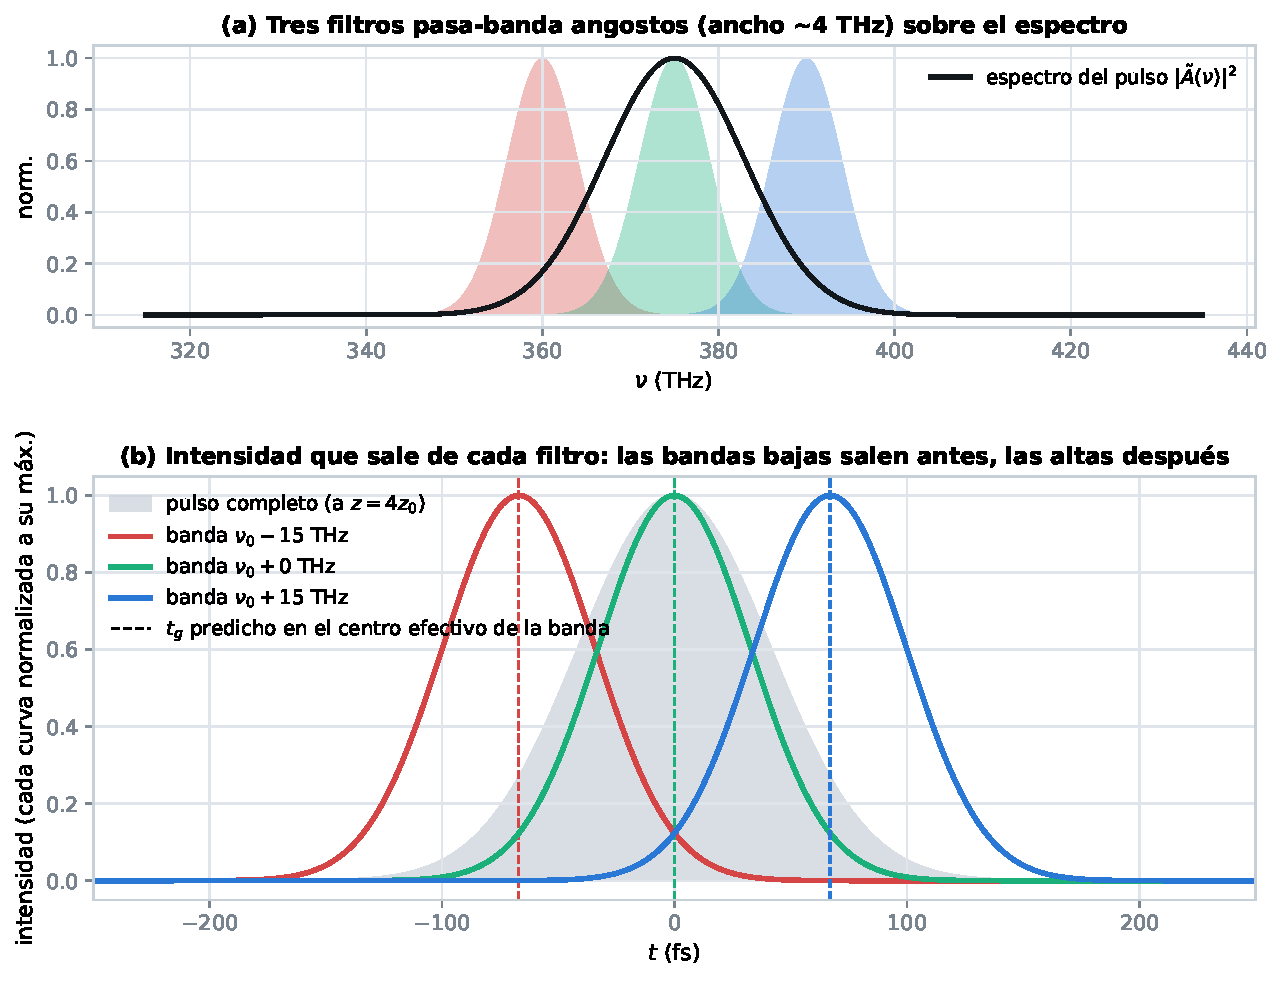
\includegraphics[width=\linewidth]{figuras/fig05_prueba_del_filtro.pdf}
\caption{Prueba del filtro sobre el pulso a $z=4z_0$. (a) Espectro y tres filtros pasa-banda. (b) Intensidad que sale de cada filtro (cada curva normalizada a su máximo); las rayas son el retardo de grupo $t_g$ predicho.}\label{fig:filtro}
\end{figure}

\begin{clave}[title={Resolución de la objeción de la «onda eterna»}]
«La frecuencia $\nu$ llega en $t_g(\nu)$» significa: \emph{el paquete formado por las frecuencias cercanas a $\nu$ está centrado en $t_g(\nu)$}. No se refiere a una onda monocromática aislada. Y hay un límite: un filtro de ancho $\delta\nu$ da un paquete de duración $\gtrsim1/\delta\nu$; cuando $\delta\nu\to0$ el paquete se vuelve infinito (la onda eterna) y la hora de llegada deja de estar definida. Aquí, con $\sigma_f=4$ THz, los paquetes duran unas decenas de fs y por eso se solapan en la Fig.~\ref{fig:filtro}b.
\end{clave}

%=====================================================================
\section{Para profundizar: la distribución tiempo--frecuencia}
%=====================================================================
Las dos descripciones, $\nu_i(t)$ y $t_g(\nu)$, se pueden dibujar juntas en el plano $(t,\nu)$. Para un gaussiano con chirp existe una distribución exacta (la de Wigner),
\[
W(t,\nu)=\sqrt{2\pi}\,\tau\;e^{-2t^2/\tau^2}\,\exp\!\big[-2\pi^2\tau^2\big(\nu-\nu_i(t)\big)^2\big],
\]
que es positiva en este caso, tiene a $I(t)=e^{-2t^2/\tau^2}$ como marginal en el tiempo y a $|\tilde A(\nu)|^2$ como marginal en la frecuencia (Fig.~\ref{fig:wigner}). Es una elipse inclinada:

\begin{itemize}
\item Dado $t$, la frecuencia media es exactamente $\nu_i(t)=\nu_0+bt/\pi$: la recta de pendiente $b/\pi$ en el plano $(t,\nu)$.
\item Dado $\nu$, el tiempo medio es $t_g(\nu)$: otra recta, de pendiente $\dfrac{1+a^2}{\pi\tau^2a}=\dfrac{b}{\pi}\dfrac{1+a^2}{a^2}$.
\end{itemize}

Las dos rectas \textbf{no coinciden salvo si $|a|\gg1$}. Para el problema 7 ($a=2$) las pendientes son $1.59$ y $1.99$ THz/fs, una razón de $(1+a^2)/a^2=1.25$. Es el mismo fenómeno que el de las dos rectas de regresión de una nube de puntos elíptica: el producto de las pendientes es el cuadrado del coeficiente de correlación,
\[
\frac{d\nu_i}{dt}\cdot\frac{dt_g}{d\nu}=\frac{a^2}{1+a^2}=r^2 .
\]
Cuando el chirp es grande ($r\to1$) la elipse se aplana sobre una recta y «qué frecuencia domina en $t$» y «cuándo llega la frecuencia $\nu$» describen lo mismo (como en la prueba del filtro a $z=4z_0$, $a=4$: $r^2=0.94$). Con chirp pequeño la elipse es casi horizontal: sin chirp, todas las frecuencias ocupan el mismo intervalo y $\nu_i(t)$ es plana.

\begin{figure}[H]\centering
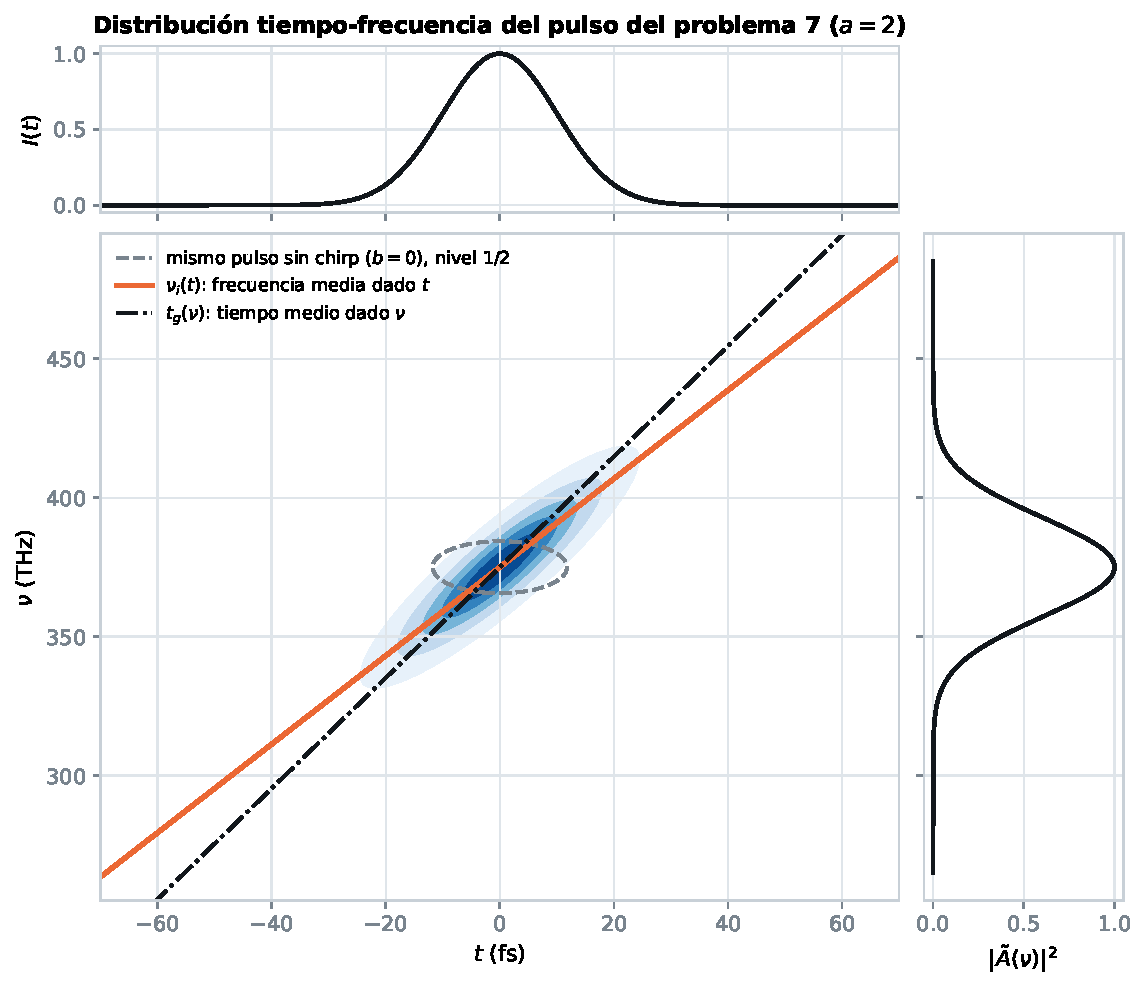
\includegraphics[width=0.85\linewidth]{figuras/fig06_distribucion_tiempo_frecuencia.pdf}
\caption{Distribución tiempo--frecuencia del pulso del problema 7. La elipse azul es $W(t,\nu)$; la elipse discontinua gris es la del mismo pulso sin chirp (misma duración, espectro $\sqrt5$ veces más angosto). Las rectas son $\nu_i(t)$ (naranja) y $t_g(\nu)$ (negra, punto-raya). Arriba: $I(t)$; a la derecha: $|\tilde A(\nu)|^2$.}\label{fig:wigner}
\end{figure}

Esta sección es de profundización: para el examen bastan las secciones 3, 4 y 6 y la idea de que el chirp es la dependencia temporal de $\nu_i$.

%=====================================================================
\section{Resumen y errores frecuentes}
%=====================================================================
\begin{center}
\renewcommand{\arraystretch}{1.35}
\begin{tabular}{@{}p{0.27\linewidth}p{0.33\linewidth}p{0.3\linewidth}@{}}
\toprule
\textbf{Concepto} & \textbf{Qué es} & \textbf{Fórmula (problema 7)}\\\midrule
Espectro $|\tilde A(\nu)|^2$ & Qué frecuencias hay en total & ancho $\propto\sqrt{1+a^2}/\tau$\\
Fase espectral $\psi(\nu)$ & Dónde se refuerzan las componentes (el «cuándo») & $-\pi^2\tau^2a(\nu-\nu_0)^2/(1+a^2)$\\
Frecuencia instantánea $\nu_i(t)$ & Oscilación local del campo total & $\nu_0+bt/\pi$\\
Retardo de grupo $t_g(\nu)$ & Hora de llegada de una banda estrecha & $\pi\tau^2a(\nu-\nu_0)/(1+a^2)$\\
Parámetro de chirp $a$ & Cuánto cambia $\nu_i$ dentro del pulso & $a=b\tau^2=2$\\
Barrido $\Delta\nu_i$ & $\nu_i(\tau)-\nu_i(-\tau)$ & $2b\tau/\pi=63.7$ THz\\
\bottomrule
\end{tabular}
\end{center}

\subsection*{Errores frecuentes}
\begin{enumerate}
\item \textbf{Imaginar que $\nu_i(t)$ es una onda monocromática que llega en $t$.} Es una propiedad de la suma, no de una componente.
\item \textbf{Confundir $\nu_0$ con $\nu_i(t)$.} $\nu_0$ es el centro del espectro; $\nu_i(t)$ es local.
\item \textbf{Creer que chirp es ensanchamiento.} El chirp es la fase; el ensanchamiento es lo que le pasa a un pulso con chirp en un medio dispersivo, y puede ser compresión si el signo es el contrario.
\item \textbf{Esperar que el chirp cambie la duración.} En el vacío no cambia nada al propagar; el chirp inicial sí ensancha el \emph{espectro} en $\sqrt{1+a^2}$.
\item \textbf{Olvidar el signo de la convención.} Con $e^{-i\omega t}$ (Boyd, Agrawal) la fase del mismo campo real lleva signo opuesto y el signo de $a$ que indica up-chirp se invierte; la física no cambia: $\nu_i$ crece con $t$.
\end{enumerate}

\end{document}
